\section{Nuvem}
O paradigma que veio a ser conhecido como \textbf{Computação em Nuvem} surgiu da confluência de interesses diversos.
\\ Por parte dos provedores, havia (1) a constatação de que infraestruturas mantidas \textit{in house} para a implantação de aplicações comerciais ficam subutilizadas na maior parte do tempo(mesmo aqueles serviços de larga escala), representando portanto um desperdício de recursos. Além disso, (2) tornava-se cada vez mais evidente a demanda por serviços que terceirizassem tarefas de montagem e manutenção de infraestrutura de forma barata, dado que tais custos representavam uma grande barreira para a implantação e oferta de aplicações de software por pequenos empreendedores e \textit{startups}.
\\ Os consumidores dessas aplicações, por sua vez, (3) demandavam o acesso a serviços de software que aproveitassem a disponibilidade de acesso à Internet para que suas funcionalidades e seus dados estivessem disponíveis em qualquer ambiente no qual eles os acessassem.
\\\\ A computação em nuvem, de maneira geral, atende a essas demandas através do fornecimento de recursos computacionais(hardware e software) como serviços acessados via rede\cite{wikiCloud}: a primeira levou à solução de particionar recursos de hardware para diferentes usos a fim de aproveitar ao máximo as capacidades daquela plataforma; a segunda motivou a criação de serviços que disponibilizam infraestrutura de hardware e software compartilhada a baixo custo via acesso remoto; a terceira, por fim, foi atendida pelo surgimento do modelo de \textit{Software como Serviço} descrito a seguir.

\subsection{Modelos de serviço}
Os serviços de computação em nuvem diferem em seu escopo e público-alvo. Essas categorias em que se classificam os serviços de nuvem são conhecidas como \textit{modelos de serviço}.Os principais modelos de serviços em nuvem são\cite{wikiCloud}:
\begin{itemize}
	\item
	\textbf{Infraestrutura como Serviço}(\textit{IaaS}): este é o modelo de serviço em nuvem mais básico. Aqui o serviço consiste em fornecer acesso a máquinas físicas ou, o que é mais comum, a instâncias de máquinas virtuais e outros recursos. Os usuários acessam essas máquinas remotamente e instalam o ambiente de software necessário para o seu consumo. O serviço é responsável por controlar o acesso aos recursos computacionais do sistema de nuvem de acordo com a necessidade e cobrar de acordo com o uso(por exemplo, se o cliente necessita de mais poder computacional, o sistema pode disponibilizar núcleos de processamento adicionais e cobrar pelo uso deles). Serviços que se encaixam nessa categoria incluem \textbf{Amazon EC2}, \textbf{Windows Azure} e \textbf{Google Compute Engine};
	\item
	\textbf{Plataforma como Serviço}(\textit{PaaS}): no modelo PaaS os provedores fornecem uma \textbf{plataforma de desenvolvimento e implantação} que inclui um sistema operacional, sistema de gerenciamento de banco de dados, servidor web, etc. Os usuários desses serviços são desenvolvedores de software que desejam desenvolver e implantar sistemas sem arcar com os custos de tempo e dinheiro associados à compra, montagem e manutenção dessa plataforma necessária para o desenvolvimento e oferta do sistema.
	\item
	\textbf{Software como Serviço}(\textit{SaaS}): o modelo de software como serviço é caracterizado pela oferta de \textbf{funcionalidades de software} em uma infraestrutura de nuvem online. Os usuários não precisam gerenciar a estrutura do provedor de nuvem para acessar o serviço: eles apenas enxergam a funcionalidade da aplicação. O modelo apresenta uma série de vantagens para os fornecedores e clientes do serviço:
	
	\begin{itemize}
		\item
		O serviço é facilmente escalável, bastando replicar o serviço em várias máquinas diferentes e usar um \textit{load balancer} para definir em tempo de execução qual máquina provê o serviço a cada cliente;
		\item
		A logística de atualiações de software é drasticamente simplificada, pois as atualizações só precisam ser aplicadas na infraestrutura de nuvem que abriga o serviço;
		\item
		Os clientes podem acessar o serviço sem precisar instalar programas adicionais em suas máquinas e têm seus dados do serviço disponíveis em qualquer ambiente em que eles o acessarem.
	\end{itemize}
	
	Exemplos de serviços em nuvem populares que seguem o modelo SaaS são \textit{Google Docs} e \textit{OnLive}.
\end{itemize}
O relacionamento entre esses modelos está ilustrado na figura \ref{fig:CloudModels}(retirada de \cite{wikiCloud})\\

\begin{figure}[h]
	\centering
    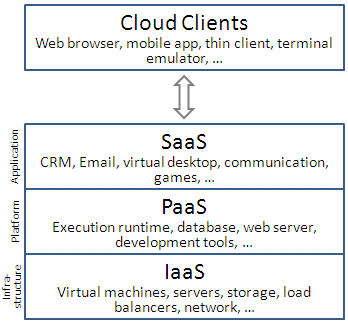
\includegraphics[scale=0.50]{figuras/Cloud_computing_layers.png}
    \caption{Modelos de serviço em nuvem}
    \label{fig:CloudModels}
\end{figure}

Outros modelos que não serão abordados em detalhes são \textbf{Rede como Serviço}(\textit{NaaS}), \textbf{Armazenamento como Serviço}(\textit{STaaS}), \textbf{Dados como Serviço}(\textit{DaaS}), \textbf{Virtualização de Desktops}, entre outros.
